\documentclass[a4paper,12pt]{article}

\usepackage{fontspec}
\setmainfont{Times New Roman}
\usepackage[russian]{babel}
\usepackage{graphicx, float, url}
\usepackage{geometry}
\geometry{left=3cm,right=1.5cm,top=2cm,bottom=2cm}
\usepackage{setspace}
\onehalfspacing
\setlength{\parindent}{1.25cm}

\begin{document}

\begin{titlepage}
  \thispagestyle{empty}
  \begin{center}

    
\includegraphics[width=0.18\textwidth]{../assets/gerb.png} \vspace{0.5cm}

    {\small
      МИНИСТЕРСТВО НАУКИ И ВЫСШЕГО ОБРАЗОВАНИЯ\\
      РОССИЙСКОЙ ФЕДЕРАЦИИ
    }

    \vspace{0.3cm}

    {\small
      Федеральное государственное бюджетное образовательное учреждение\\
      высшего образования
    }

    \vspace{0.3cm}

    {\large \textbf{«МИРЭА --- Российский технологический университет»}}

    {\normalsize РТУ МИРЭА}

    {\normalsize Институт искусственного интеллекта (ИИИ)}\\
    {\normalsize Кафедра промышленной информатики (ПИ)}

    \vspace{2cm}

    {\LARGE \textbf{ОТЧЁТ}}

    \vspace{0.3cm}

    {\Large \textbf{ПО ПРАКТИЧЕСКОЙ РАБОТЕ № 15}}

    \vspace{0.4cm}

    {\large по дисциплине «Информатика»}

    \vspace{2.5cm}

    \begin{tabular}{ll}
      Выполнил студент группы КВБО-11-25 & Шапаренко Ф.А. \\
      Принял ассистент: & Беднов Г.А. \\
    \end{tabular}

    \vfill

    Практическую работу выполнил: «05» апреля 2026 г.\\
    «Зачтено» \rule{1cm}{0.4pt} 2026 г.

    \vspace{1cm}

    Москва 2026

  \end{center}
\end{titlepage}

\noindent\textbf{Тема:} «Элементарная ячейка памяти»\\
\noindent\textbf{Цель работы:} \\ -  освоение принципов построения
и режимов работы асинхронных  триггеров;  \\ -  освоение принципов
построения и режимов работы синхронных  триггеров со статическим
управлением;  \\ -  изучение режимов работы синхронных триггеров с
динамическим управлением.  \\ -  ознакомление с принципом работы
ячейки памяти;  \\ -  исследование влияния управляющих сигналов на
работу  ячейки памяти;  \\ -  реализация и исследование ячейки памяти
на основе  триггеров.

\url{https://simulator.io/board/geHoS6NABk/1}

\begin{figure}[H]
  \begin{center}
    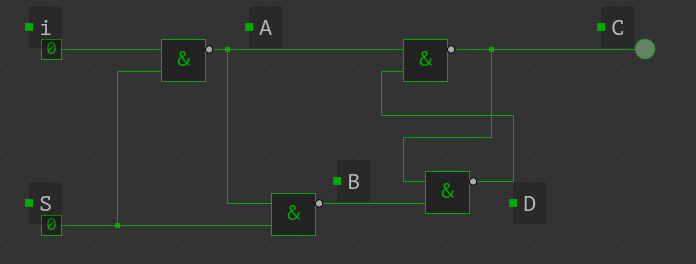
\includegraphics[width=0.95\textwidth]{../assets/15.png}
  \end{center}
  \caption{Схема}
\end{figure}

\begin{table}[H]
  \centering
  \large
  \caption{Таблица истинности}
  \begin{tabular}{|c|c|c|}
    \hline
    i & S & C \\ \hline
    0 & 0 & C \\ \hline
    0 & 1 & 0 \\ \hline
    1 & 0 & C \\ \hline
    1 & 1 & 1 \\ \hline
  \end{tabular}
\end{table}

\end{document}
